%
% Gas Target NIM Paper 
%
% Updated 17 November 2018 by Higinbotham
%
%\documentclass[preprint,12pt]{elsarticle}

%% Use the option review to obtain double line spacing
%% \documentclass[authoryear,preprint,review,12pt]{elsarticle}

%% Use the options 1p,twocolumn; 3p; 3p,twocolumn; 5p; or 5p,twocolumn
%% for a journal layout:
%% \documentclass[final,1p,times]{elsarticle}
%\documentclass[final,1p,times,two]{elsarticle}
%% \documentclass[final,3p,times]{elsarticle}
%% \documentclass[final,3p,times,twocolumn]{elsarticle}
%% \documentclass[final,5p,times]{elsarticle}
%%\documentclass[final,5p,times,twocolumn,balance]{elsarticle}

\documentclass[final,5p,times,twocolumn]{elsarticle}
\usepackage{amsmath, amssymb, amsfonts, latexsym}
\usepackage{subcaption}
\usepackage{adjustbox}
\usepackage{graphicx}

%% For including figures, graphicx.sty has been loaded in
%% elsarticle.cls. If you prefer /to use the old commands
%\usepackage{epsfig}
%\usepackage{mathtools}
%\usepackage{xcolor}
%\usepackage{textcomp}
%\usepackage{balance}
%\usepackage[LGRgreek]{mathastext}
%% The amsthm package provides extended theorem environments
%% \usepackage{amsthm}
%% The lineno packages adds line numbers. Start line numbering with
%% \begin{linenumbers}, end it with \end{linenumbers}. Or switch it on
%% for the whole article with \linenumbers.
%% \usepackage{lineno}

\journal{Nuclear Instruments and Methods}

\begin{document}

\begin{frontmatter}

%% Title, authors and addresses
%% use the tnoteref command within \title for footnotes;
%% use the tnotetext command for theassociated footnote;
%% use the fnref command within \author or \address for footnotes;
%% use the fntext command for theassociated footnote;
%% use the corref command within \author for corresponding author footnotes;
%% use the cortext command for theassociated footnote;
%% use the ead command for the email address,
%% and the form \ead[url] for the home page:
%% \title{Title\tnoteref{label1}}
%% \tnotetext[label1]{}
%% \author{Name\corref{cor1}\fnref{label2}}
%% \ead{email address}
%% \ead[url]{home page}
%% \fntext[label2]{}
%% \cortext[cor1]{}
%% \address{Address\fnref{label3}}
%% \fntext[label3]{}

\title{Density Changes in Low Pressure Gas Targets for Electron Scattering Experiments}
%\title{Performance of the Hall A Tritium Target}

\author[UNH]{S.~N.~Santiesteban}
\author[Kent]{S.~Alsalmi}
\author[JLab]{D.~Meekins}
\author[TN]{J.~Bane}
\author[WM]{S.~Barcus}
\author[SM]{J.~Campbell}
\author[FI]{J.~Castellanos}
\author[MIT]{R.~Cruz-Torres}
\author[VT]{H.~Dai}
\author[Kent]{T.~Hague}
\author[OD]{F.~Hauenstein}
\author[JLab]{D.~W.~Higinbotham\corref{cor1}}
\author[argonne,CalTech]{R.~J.~Holt}
\author[SB]{T.~Kutz}
\author[UNH]{S.~Li}
\author[COL]{H.~Liu}
\author[JLab]{R.~E.~McClellan}
\author[Kent]{M.~Nycz}
\author[UVa]{ D.~Nguyen}
\author[hampton]{B.~Pandey}
\author[VT]{V.~Pandey}
\author[MIT]{A.~Schmidt}
\author[Kent]{Tong~Su}
\author[argonne]{Z.~Ye}

\cortext[cor1]{Corresponding Author: doug@jlab.org}

\address[UNH]{University of New Hampshire, Durham, New Hampshire 03824, USA}
\address[Kent]{Kent State University, Kent, Ohio 44240, USA}
\address[JLab]{Jefferson Lab, Newport News, Virginia 23601 USA}
\address[TN]{The University of Tennessee, Knoxville, Tennessee 37996, USA}
\address[WM]{The College of William and Mary, Williamsburg, Virginia 23187, USA}
%\address[DH]{Dalhousie University, Halifax, Nova Scotia, Canada}
\address[SM]{Saint Mary's University, Halifax, Nova Scotia, Canada}
\address[FI]{Florida International University, Miami, Florida 33199 USA}
\address[MIT]{Massachusetts Institute of Technology, Cambridge, Massachusetts 02139, USA}
\address[VT]{Center for Neutrino Physics, Virginia Tech, Blacksburg, Virginia 24061, USA}
\address[OD]{Old Dominion University, Norfolk, Virginia 23529, USA}
\address[CalTech]{Kellogg radiation Laboratory, California Institute of Technology, Pasadena California 91125 USA}
\address[argonne]{Physics Division, Argonne National Laboratory, Argonne, Illinois 60439, USA}
\address[COL]{Columbia University, New York, New York 10027, USA}
\address[SB]{Stony Brook University, Stony Brook, New York 11794, USA}
\address[UVA]{Department of Physics, University of Virginia, Charlottesville, Virginia 22904, USA}
\address[hampton]{Hampton University, Hampton, Virginia 23669, USA}

\begin{abstract}
A system of modular sealed gas target cells has been developed for use in electron scattering experiments 
at the Thomas Jefferson National Accelerator Facility (Jefferson Lab). This system was initially developed 
to complete the MARATHON experiment which required, among other species, tritium as a target material. 
The system has been used in several of the 12 GeV era experiments in Experimental Hall A using the Jefferson Lab 
Continuous Electron Beam Accelerator Facility (CEBAF). Thus far, the cells have been loaded with the gas 
species $^{3}$H, $^{3}$He, $^{2}$H, $^{1}$H and $^{40}$Ar and operated in nominal beam currents of up to $22.5$ $\mu A$.  
Each cell is $25$ $cm$ long with a diameter of $1.3$ $cm$. While gas density of the cells at the time of loading is known, 
the density of the each gas varies uniquely when heated by the electron beam. To extract experimental cross sections using 
these cells the beam current dependent density of each target fluid must be determined. In this study, data from measurements 
with several beam currents within the range of $2.5$ to $22.5$ $\mu A$ on each target fluid are presented. Additionally, 
expressions for the beam dependent fluid density of each target are developed.
\end{abstract}

\begin{keyword}
Density \sep target system
\sep tritium
\sep helium 
\sep deuterium
\sep hydrogen
\sep argon
%% keywords here, in the form: keyword \sep keyword
%% PACS codes here, in the form: \PACS code \sep code
%% MSC codes here, in the form: \MSC code \sep code
%% or \MSC[2008] code \sep code (2000 is the default)
\end{keyword}
\end{frontmatter}

%% \linenumbers

%% main text
\section{Introduction}
\label{}
%%%%%

A modular gas cell target system was developed for use in Hall A at Jefferson Lab for the MARATHON experiment (E12-10-103)\cite{marathon}. The design was specifically developed to safely contain and operate with gaseous tritium~\cite{Brajuskovic:2013ymh}. The modular design allows additional gas cells filled with other species of gas to be installed in the system concurrently. The target was also adapted for the additional experiments E12-11-112 ($x_{b}>1$) \cite{E12-11-112}, E12-14-011 ($e'p$) \cite{E12-14-011}, E12-17-003 (Hypernuclear) \cite{hypernuclear} and E12-14-009 (elastic) \cite{E12-14-009}.  MARATHON, together with these experiments, became known as the tritium group experiments which were performed from December 2017 through November 2018. However, prior to tritium operations, a target cell was loaded with argon gas and used by the experiment E12-14-012 (Argon) \cite{E12-14-012} during Spring of 2017. 

While the performance of the target was an important consideration, the primary objective of the target system design and construction was to ensure safe operations with tritium gas under all conditions including reasonable upset conditions. These conditions included target cell preparations, loading, storage, transportation, installation, removal, and beam operations. This was accomplished with a modular design, rigorous fabrication and testing, proper quality assurance (QA) and quality control (QC) and multiple layers of containment/confinement. 
 
In addition to a brief description of the target, we present the beam current dependent density of the five gases used 
with the target system, $^{3}$H, $^{3}$He, $^{2}$H, $^{1}$H and $^{40}$Ar. The electrons in the beam pass through the target fluid and cell entrance and exit end caps depositing ionization energy. This ionization energy, which is proportional to the beam current, induces heat in the target fluid causing local changes in the density. To determine the magnitude of this effect, data were collected with the Left High Resolution Spectrometer (LHRS) in Jefferson Lab Experimental Hall A during February 2017 for the $^{40}$Ar target and December 2017 for the other targets. The beam energy for the study was $2.2$ GeV in all cases, The momentum and angle settings were $17.5 ^\circ $ and $1.79$ GeV for $^{40}$Ar, and $17.0 ^\circ $ and $1.99$ GeV for the other fluids. Analysis of these data shows that a simple quadratic polynomial function normalized to zero current density provides an excellent model for all target fluids.


\section{Target System}

The modular design allows multiple cell configurations. It also enables individual cells to be installed in special configurations of the standard Hall A Cryogenic target; this was the case for the $^{40}$Ar target (see Figure \ref{argon}). Another feature is that it allows cells to be filled at off site locations other instead of Jefferson Lab. The tritium cell was filled at Savannah River Site (SRS) by Savannah River Tritium Enterprises (SRTE). The tritium cell was filled with about 0.1 grams of tritium gas to a room temperature pressure of about 200 psia. It was shipped in a special purpose transport container called the Bulk Tritium Shipping Package (BTSP). Including the cell this system provided continuous triple layer confinement though out the shipping and handling process. This design also allowed the tritium cell to be stored in a special storage container in Hall A while normal Hall installation activities were completed. The tritium cell was installed after all other preparatory tasks were completed.

\begin{figure}[htbp]
	\centering
	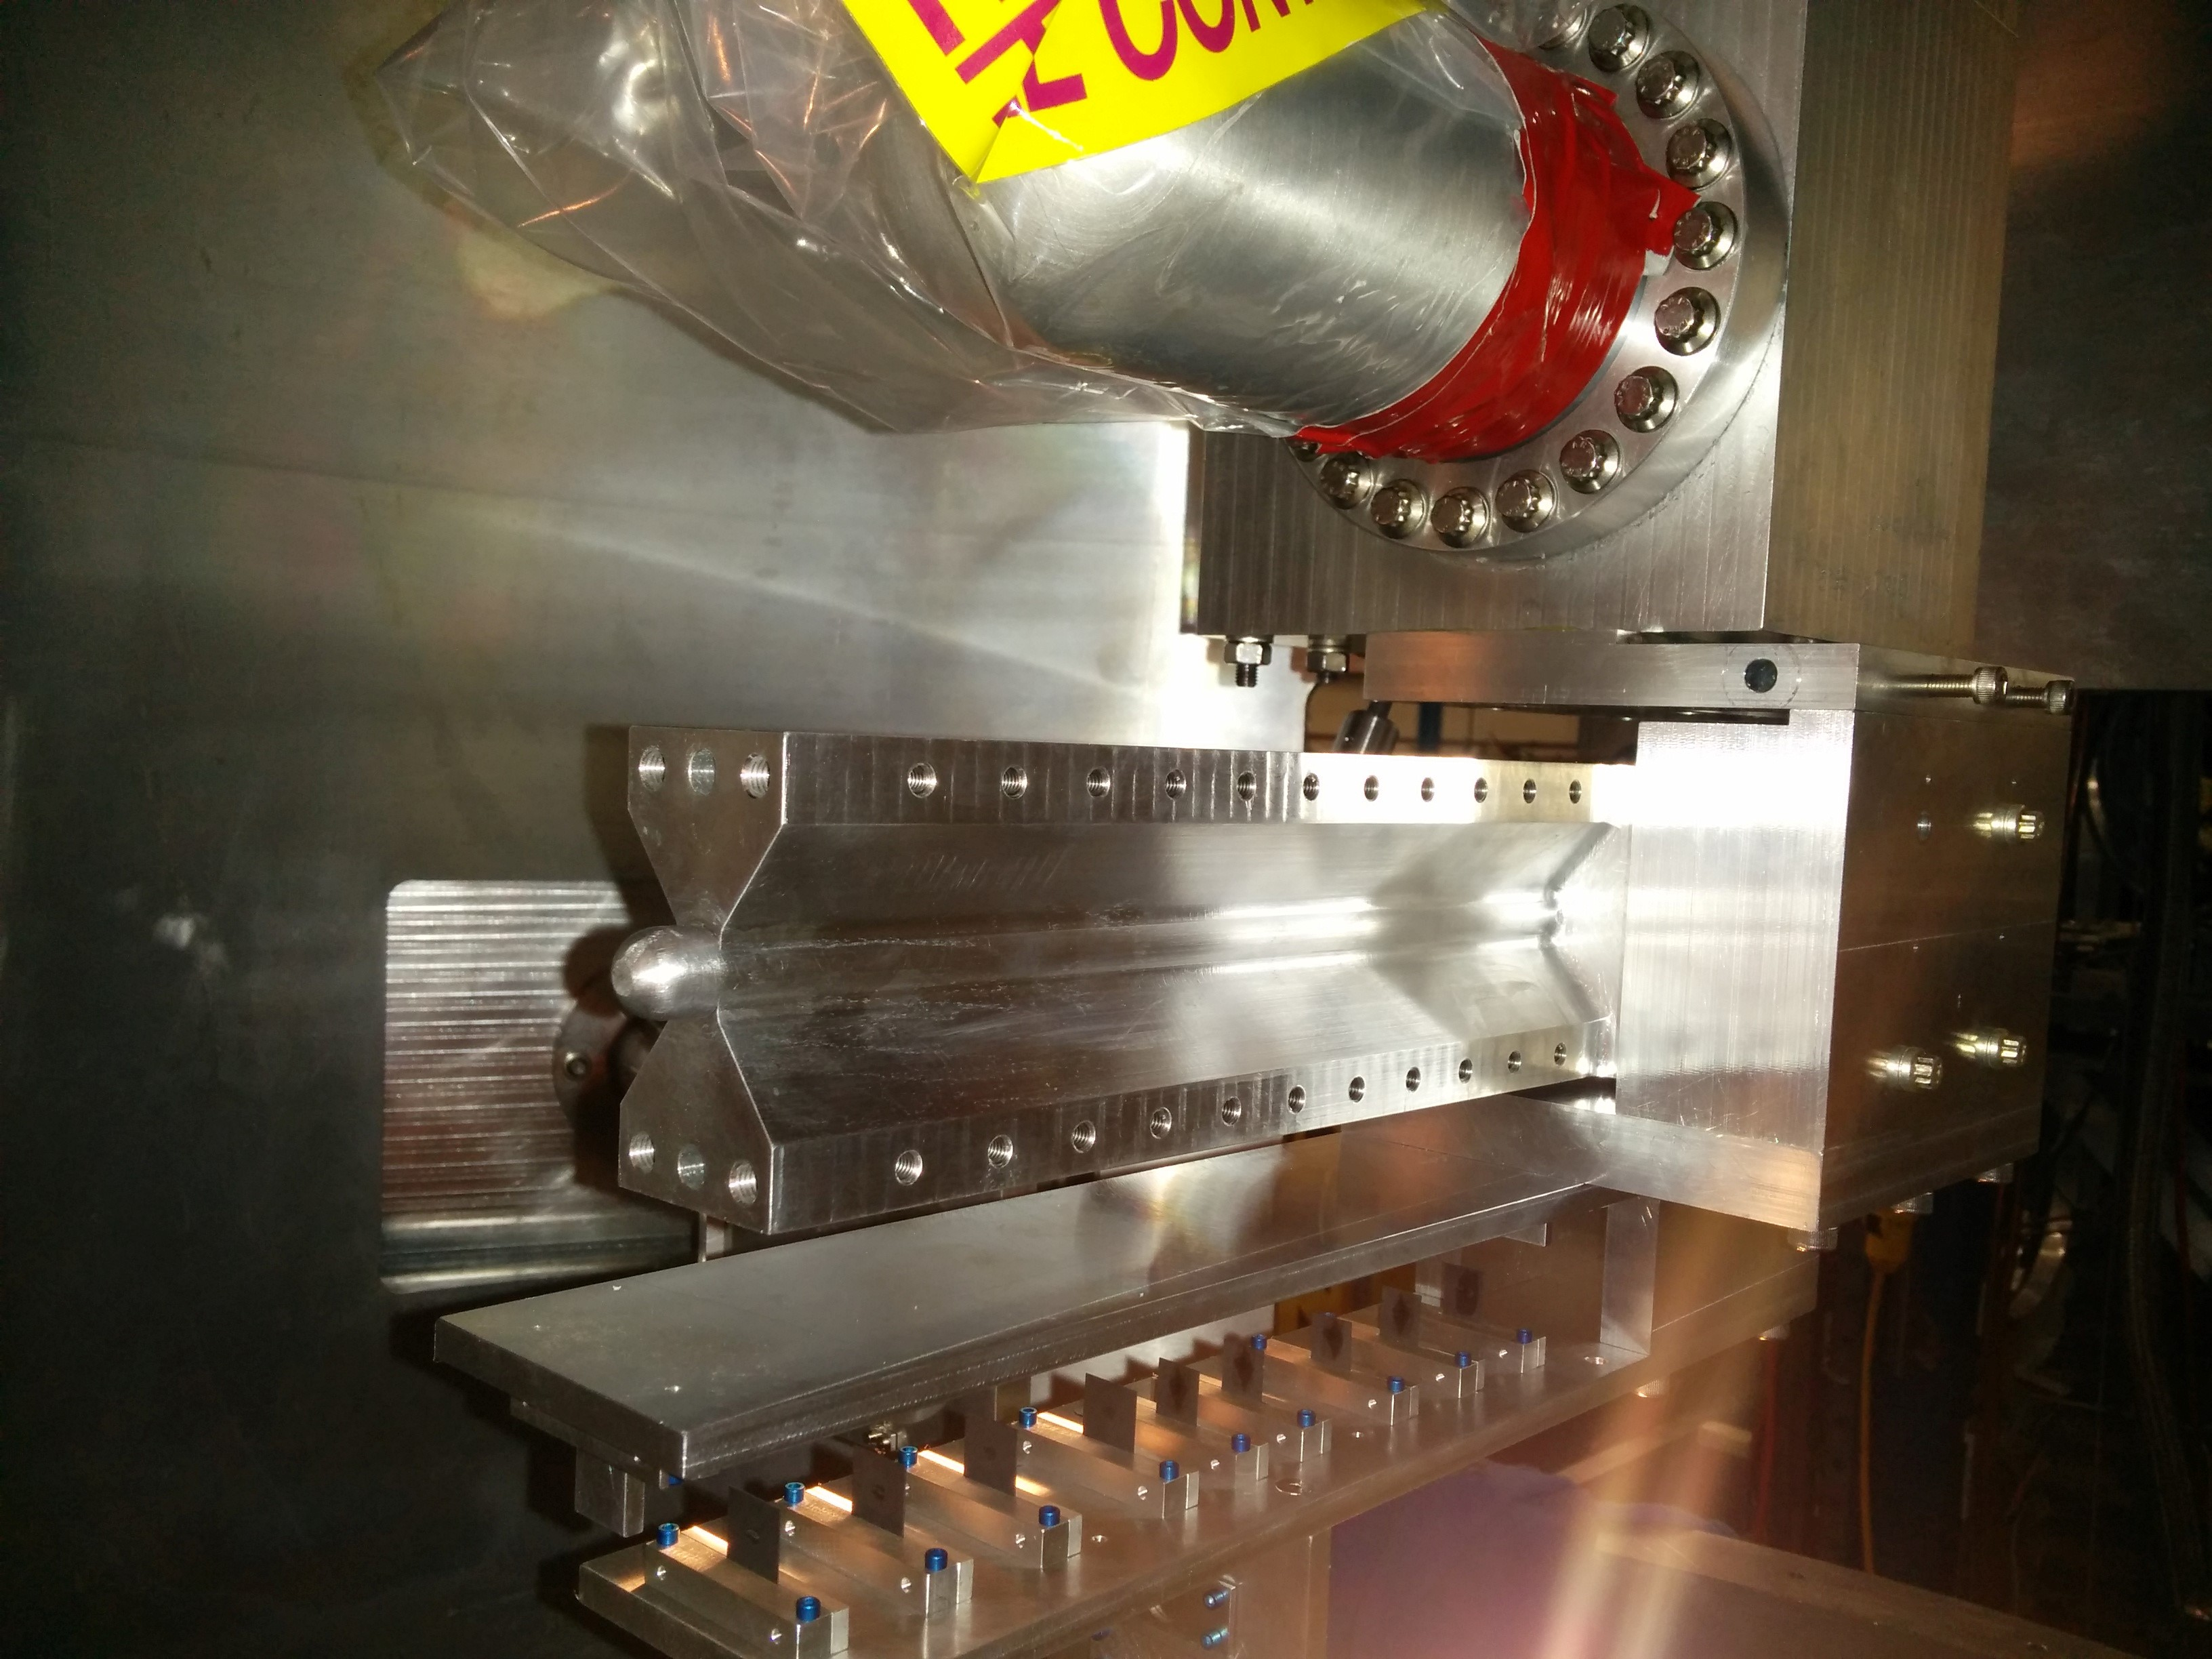
\includegraphics[width=6.5 cm]{images/Ar-cell.jpg}\\
	\caption{Argon cell installation. A cell filled with $^{40}$Ar was installed on the standard Hall A Cryogenic Target in place of the loop 3 cell.}
	\label{argon}
\end{figure}

\begin{figure}[htbp]
  \centering
  % Se pueden incluir figuras jpeg al compilar con PDFLatex
  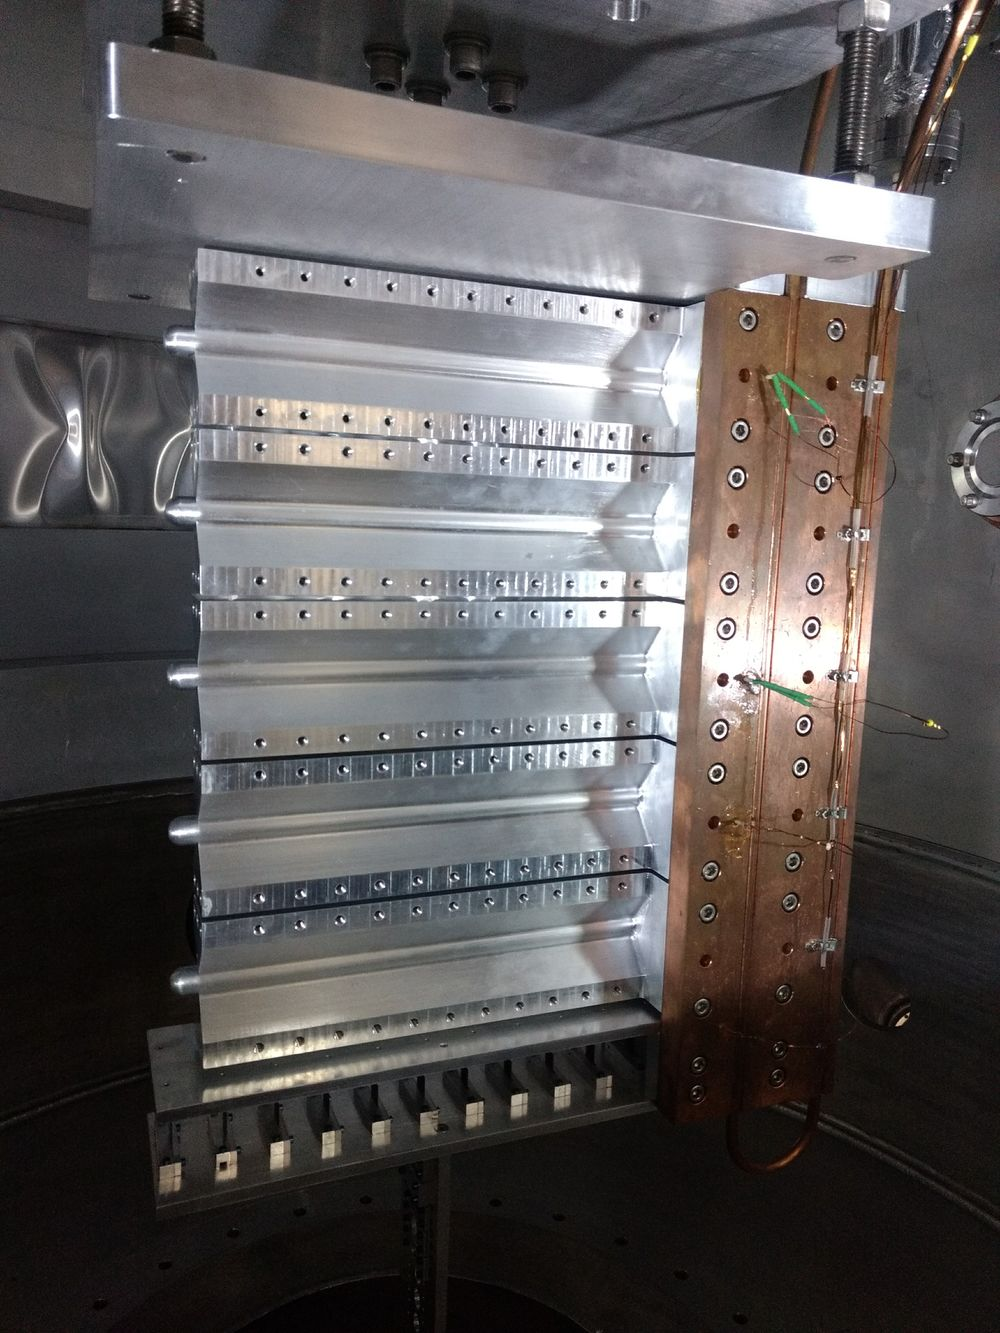
\includegraphics[width=6.5cm]{images/ladder.jpg}\\
  \caption{Ladder Assembly. Five cells were assembled during Fall 2017 to Spring 2018, $^{3}H$, $^{2}H$, $^{1}H $, $^{3}He$ and empty cell from top to bottom.}
  \label{ladder}
\end{figure}

The configuration of the tritium target is shown in Figure \ref{ladder}. In this configuration, there are (from top to bottom) four cells loaded with $^{3}$H, $^{2}$H, $^{1}$H, and $^{3}$He as well as a fifth empty cell which was used for background measurements. The cells are contained in a scattering chamber which is under vacuum. The scattering chamber vacuum is isolated from the upstream beam line vacuum by a 0.2 mm thick beryllium window. This window is roughly 30 cm upstream of the target center and is mounted on a reentrant tube that also contains a $15$ $cm$ long tungsten collimator with an inner diameter of 12.7 mm. The target vacuum, with a pumping system directed to an exhaust stack, provided a second layer of tritium confinement. An exhaust system, (together with strict access controls) capable of maintaining a slight negative pressure in the experimental Hall ensured that the Hall boundary was a third layer of confinement.

Each cell, excluding the fill valve assembly, is machined from ASTM B209 aluminum 7075-T651 plate. Each target cell has a cigar-tube shaped active fluid space with a length of $25$ $cm$ and a diameter of $12.7$~$mm$. The total volume of the cell (including the non active region) is $33.38 \pm 0.2$ cm$^{3}$. The thickness of the nearly flat entrance window and hemispherical exit window is nominally $0.25$ $mm$. The parameters at the time of loading for each cell are summarized in Table \ref{tab:fill_tar}. Due to machining tolerances, the wall thickness of each cell varies slightly over its length. Thickness measurements were performed for each cell at several locations (schematically represented in Figure~\ref{fig:cellconfig} and are summarized in Table \ref{cell}. The $^{40}$Ar cell, installed in February 2017 in a special configuration, was later installed as the empty (or dummy) cell for the tritium group of experiments. Table \ref{tab:cell} shows the $^{40}$Ar and the Empty Cell in a single column. The $^{40}$Ar experiment employed two aluminum foils (dummy target), with total thickness matching the radiation length of the argon filled cell, to measure backgrounds.

The entire target assembly, of five cells and assorted solid targets, was cooled with $15K$ helium from the Jefferson Lab End Station Refrigerator (ESR). The $15K$ helium was preheated to $40K$ and used to cool a heat sink to which the cell assemblies were attached. This removed the modest amount of heat generated by the electron beam passing through the target fluid, cell entrance and cell exit, which, in total, was about $15W$. To ensure cell integrity, the maximum beam current permitted on any of the cells was $22.5$ $\mu A$ \cite{engreport}. The heat generated by the tritium decay is very small, about $50$ $mW$ and was negligible.

%The target thickness values of this table are changed with the beam current and ultimately the percentage changed in the density will be applied as a correction factor to this values. The gas with major density used in the experiments was $^{40}$Ar and the lower density target was $^{3}H$.  Additionally, the top view of the cell is shown in Figure \ref{fig:cellconfig},  it shows the beam direction and the two windows of the cell.

\begin{table}[!h]
\centering
\begin{adjustbox}{width=0.5\textwidth}
\begin{tabular}{|c|c|c|c|}
	\hline 
	Target       & Fill Pressure & Fill Temp    & Thickness \\
	Fluid  		 &	$kPa$)		 &	($K$) 	    & ($mg/cm^2$) \\
	\hline 
	$^{40}$Ar	 & $3447$ 		 & $291$	    &  $1455\pm9.2$ \\ 
	\hline 
	$^{3}$H-1 	 & $1400$		 & $296.3$	    &  $85.1\pm 0.83$ \\ 
	\hline 
	$^{3}$H-2	 & $1393$		 & $293.8$		&  $84.79\pm0.82$ \\
	\hline
	$^{3}$He	 & $1772$		 & $294.3$	    &  $53.37\pm0.57$ \\ 
	\hline 
	$^{2}$H 	 & $3549$		 & $296.1$	    &  $142.15\pm0.80$ \\ 
	\hline 
	$^{1}$H 	 & $3549$		 & $297.4$	    &  $70.80\pm0.40$ \\ 
	\hline 
\end{tabular}
\end{adjustbox}
\caption{Load data for the gas cells. Temperatures have an uncertainty of $0.1K$. Values for the $^{40}$Ar cell are from Ref.~\cite{ar_config}; for all others they are from REF\cite{cellconfig}. }.
\label{tab:fill_tar}
\end{table}

%\begin{table}[!h]
%\centering
%\begin{adjustbox}{width=0.5\textwidth}
%\begin{tabular}{|c|c|c|c|c|}
%\hline
%Target   & Mass (mg)           & \begin{tabular}[c]{@{}c@{}}$\rho$ t (mg/cm$^{2})$\\ Target thickness\end{tabular} & \begin{tabular}[c]{@{}c@{}}Filling Pressure\\ (psia) \end{tabular} & Temperature (K)  \\ \hline
%$^{40}$Ar  & $1942.7$              & $1455$                                           & $500$ & $291$ \\ \hline
%$^{3}$H    & $102.8$              & $77 \pm 0.01$ & $203$                                                             & $291$\\ \hline
%$^{3}$He   & $ 71.3  $  & $53.4 \pm 0.6$ & $252.7$                                                           & $294.3$ \\ \hline
%$^{2}$H    & $189.86$ & $142.2 \pm 0.8$  & $514.7$                                                           & $296.1$
%\\ \hline
%$^{1}$H    & $94.53 $ & $70.8 \pm 0.4$  & $514.7$                                                          & $297.4$
%\\ \hline
%\end{tabular}
%\end{adjustbox}
%\caption{Gas target filling parameters. Temperatures have an uncertainty of $0.1\circ $. $^{40}$Ar taken from \cite{ar_config} and for the other targets from \cite{cellconfig}. }. 
%\label{tab:fill_tar}
%\end{table}

\begin{figure}[!h]
  \centering
  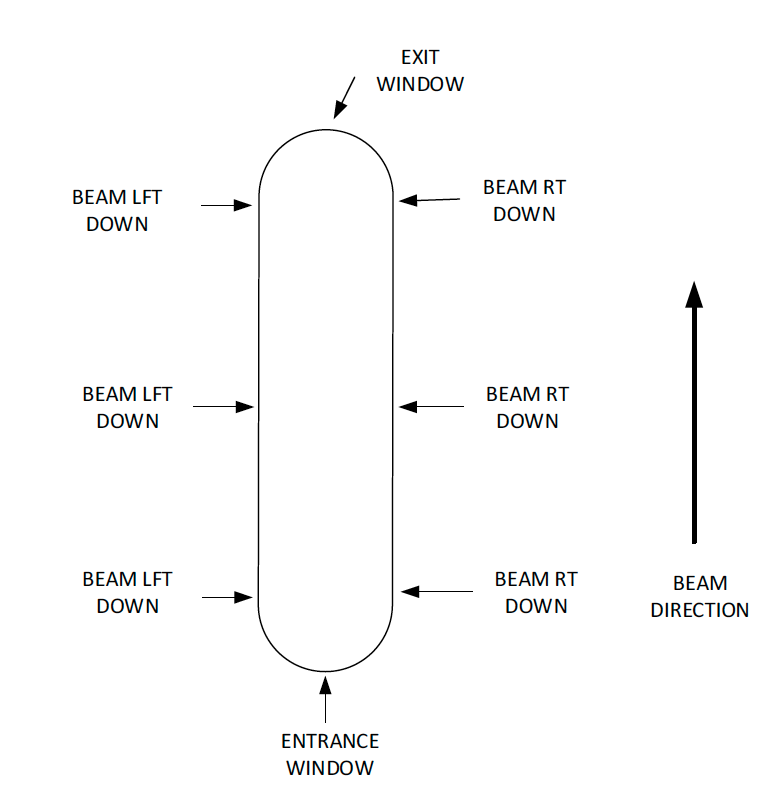
\includegraphics[width=\linewidth]{images/tgt_measurements.png}\\
  \caption{Measurement locations on the cells represented schematically \cite{cellconfig}.}
  \label{fig:cellconfig}
\end{figure}

%The gas targets are contained in a $25$ $cm$ long by $1.3$ $cm$ diameter aluminum (7075-T6) sealed system, the target cell is shown in Figure \ref{cell}. 
%The alloy 7075-T6 was chosen since it has high thermal conductivity, high yield strength, and it is used for target cells at JLab commonly. 
%The windows for beam entrance and exit were designed to be $0.0254$ $cm$ and $0.0279$ $cm$ thick, respectively \cite{celldes}. However, due to the fact that the cell was machined out of a single aluminum piece, the exit window has slightly different measurements for each target, as it is summarized in Table \ref{tab:cell}.



\begin{table*}[!h]
\centering
\begin{adjustbox}{width=1\textwidth}
\begin{tabular}{|c|c|c|c|c|c|}
\hline
Location        & \begin{tabular}[c]{@{}c@{}} $^{40}$Ar/Empty Cell\\ Thickness $(mm)$\end{tabular} & \begin{tabular}[c]{@{}c@{}}$^{3}H$ Cell\\ Thickness $(mm)$\end{tabular} & \begin{tabular}[c]{@{}c@{}}$^{1}H$ Cell\\ Thickness $(mm)$\end{tabular} & \begin{tabular}[c]{@{}c@{}}$^{2}H$ Cell\\ Thickness $(mm)$\end{tabular} & \begin{tabular}[c]{@{}c@{}}$^{3}He$ Cell\\ Thickness $(mm)$\end{tabular} \\ \hline
Entrance               &      $0.254 \pm 0.0051$                                                  & $0.253 \pm 0.004$                                                     & $0.311 \pm 0.001$                                                     & $0.215 \pm 0.004$                                                     & $0.203 \pm 0.007$                                                      \\ \hline
Exit                    &    $0.279 \pm 0.0051$                                                  & $0.343 \pm 0.047$                                                     & $0.330 \pm 0.063$                                                     & $0.294 \pm 0.056$                                                     & $0.328 \pm 0.041$                                                      \\ \hline
Exit left              &      $0.406 \pm 0.0051$                                                 & $0.379 \pm 0.007$                                                     & $0.240 \pm 0.019$                                                     & $0.422 \pm 0.003$                                                     & $0.438 \pm 0.010$                                                      \\ \hline
Exit right              &       $0.421 \pm 0.0051$                                                 & $0.406 \pm 0.004$                                                     & $0.519 \pm 0.009$                                                     & $0.361 \pm 0.013$                                                     & $0.385 \pm 0.016$                                                      \\ \hline
Mid left             &        $0.457 \pm 0.0051$                                                  & $0.435 \pm 0.001$                                                     & $0.374 \pm 0.004$                                                     & $0.447 \pm 0.009$                                                     & $0.487 \pm 0.060$                                                      \\ \hline
Mid right             &        $0.432 \pm 0.0051$                                                  & $0.447 \pm 0.004$                                                     & $0.503 \pm 0.005$                                                     & $0.371 \pm 0.012$                                                     & $0.478 \pm 0.007$                                                    \\ \hline
Entrance left      &          $0.508 \pm 0.0051$                                                  & $0.473 \pm 0.003$                                                     & $0.456 \pm 0.010$                                                     & $0.442 \pm 0.005$                                                     & $0.504 \pm 0.003$                                                      \\ \hline
Entrance right     &		 $0.424 \pm 0.0051$                             & $0.425 \pm 0.003$                                & 
$0.457 \pm 0.006$                                & 
$0.332 \pm 0.011$                                & 
$0.477 \pm 0.011$                                 \\ \hline
\end{tabular}
\end{adjustbox}
	\caption{Cell wall thickness measurements for all gas targets. Values for the $^{40}$Ar cell are from  Ref\cite{ar_config}; for all others they are from REF\cite{cellconfig}.}
	\label{tab:cell}
\end{table*}


\begin{figure*}[!h]
\centering
  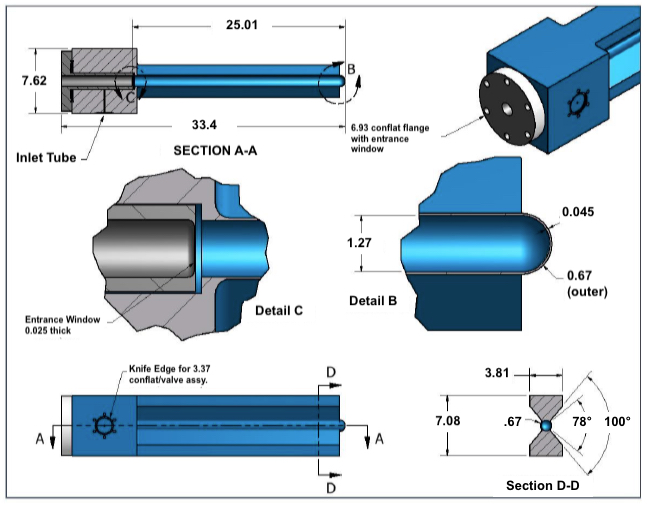
\includegraphics[width=13cm]{images/tritium_cell.jpg}\\
  %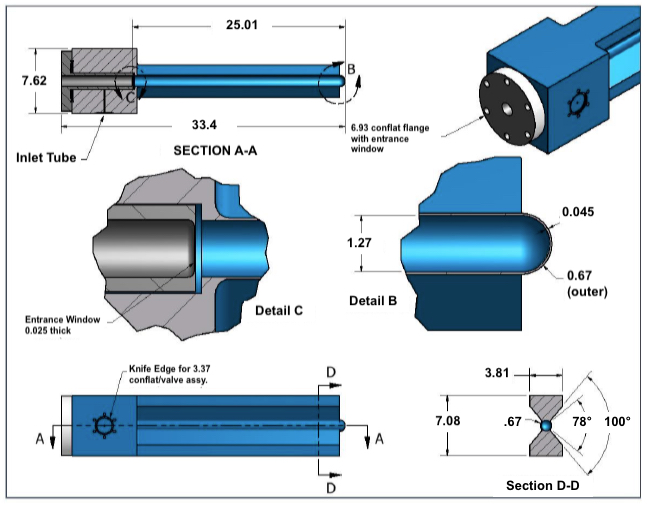
\includegraphics[width=\linewidth]{images/tritium_cell.jpg}\\
  \caption{Engineering design of an individual tritium gas target cell \cite{celldes}, units are in $cm$.
 }\label{cell}
\end{figure*}


\section{Experimental Hall A}

The data were acquired with the LHRS. For a detailed description of the LHRS see Ref \cite{Alcorn:2004sb}. The basic components of the LHRS are one non superconducting quadrupole(Q1), a super conducting quadrupole (Q2) a superconducting dipole (D) followed by a super conducting quadrupole (Q3) in a Q-Q-D-Q configuration. The quadrupoles focus scattered charged particles while the dipole directs these particles, within a given momentum range, to the detectors. After passing through the spectrometer magnets, the scattered particles pass through two Vertical Drift Chambers (VDCs), which provide tracking information. Two layers of scintillator hodoscope s0 and s2, sandwich a gas Cherenkov detector filled with CO2. The hodoscope provides trigger and time of flight (TOF) for the detected particles. The Cherenkov provides identify electrons with $99 \%$  efficiency and reject $\pi^{-}$ below momentum of $4.8$ $GeV$ . The last element in the detector stack is the shower calorimeter. Electrons pass through the calorimeter lead glass blocks induce a cascade of pair production and bremsstrahlung radiation from which their energy can be determined\cite{Alcorn:2004sb}.


\section{Beam Current Monitor (BCM)}
\label{BCM}

The Beam Current Monitor (BCM) is a system of three independent devices and a current source. This system accounts for most  
of the systematic uncertainty in the density study.  The BCM system consists of a toroidal sensor (Unser), located between 
an upstream and downstream RF cavity, and a data-acquisition system.  A current source, which is contected to a wire which 
passes through the Unser, is used to calibrate the Unser immediately prior to each use of the device and
the Unser is then in turn used to calibrate the BCM's with the electron beam. 

The Unser monitor is composed of two identical toroidal cores driven in opposite ways by an external source.  
The DC component of the current flowing through the toroid sensor is detected by a magnetic modulator. The 
beam current in the cores produces a flux imbalance, which generates an output signal proportional to the 
even harmonics of the frequency of excitation, In the absence of DC current, the sum of the signals is zero~\cite{denard}. 

The temperature controlled Unser has sensitivity to beam current of about $4$ $mV/\mu A$ and has a noise canceled 
stability within $0.1\%$~\cite{denard}.  The system does have a DC offset which slowly drifts which typically 
requires the current calibration to be done immediately prior to using it for an absolute current calibration.
of the RF cavities.  Once calibrated, the RF cavities are used to continuously monitor the beam current. 
The calibrations are checked periodically though out the course of an experiment. 
To put the signals from the Unser and RF cavities into the scalers of Hall's fast data aquitions system,
a voltage to frequency (V/F) converter is used along with a distrinater. 
Figure \ref{fig:unser_cal} shows the Unser calibration with a known DC current source, 
the response of the system is found to be $0.0002497 \pm 9.6 \times 10^{-7} $ $\mu A/Hz$. 

\begin{figure}[!h]
    \centering
    \includegraphics[width=\linewidth]{images/unser_calibration.pdf}
    \caption{Wire Unser calibration. The band reprecents the $95\%$ confidence level of the linear fit.}
    \label{fig:unser_cal}
\end{figure}
  
Two resonant cavities surround the Unser and are tuned to the frequency of the beam $1.497$ $GHz$ with a quality coefficient $Q \approx 500$. The cavities are composed of loop antennas located where the magnetic field is maximum. When the beam passes through, the output RF signal is proportional to the current \cite{denard}. As consequence, the BCM response is linear with respect to the current. Like the Unser, the signals from the RF cavities are filtered by a V/F converter. Several values of beam current (measured by the calibrated Unser) are used to the determine the linear dependence of the BCM as shown in Figure \ref{fig:dnew_cal}. In general, the beam current can be then calculated using

\begin{equation}
I = g_{BCM}\cdot f+O.
\label{eq:current_calc}
\end{equation}

\noindent Where $g_{BCM}$ and $O$ are the fit parameters, which correspond to $0.0003264 \pm 1.4 \times 10^{-6}$ $\mu A/Hz$ and $0.1 \pm 0.09$  $\mu A$, respectively. Finally, for any given beam induced frequency $f$, the current $I$ is given by Eq \ref{eq:current_calc}. Of unfortunate note, the BCM system becomes much less accurate for beam currents below $\sim 5$ $\mu A$.
  
\begin{figure}[!h]
      \centering
    \includegraphics[width=\linewidth]{images/dnew_calibration.pdf}
    \caption{BCM calibration. The band reprecents the $95\%$ confidence level of the linear fit.}
    \label{fig:dnew_cal}
\end{figure}


\section{Method Overview}

The density of the target is well known when loaded but, experience and simulations have shown that the beam current will 
decrease the density of the target fluid in the beam path (local density). The magnitude of this effect depends on the 
beam current and target fluid species and must be quantified to accurately determine cross sections and ratios or 
other comparisons of data collected with the multiple gas cells~\cite{celldes}. 
It was shown that the target density reaches equilibrium within an insignificant amount of time from when the 
electron beam first impinges on the cell and the density was constant with stable beam current. The purpose of 
these measurements and analysis is to develop a beam current dependent target density function for each gas species used.  

In order to extract the density, the raw yield is measured for several beam currents. The normalized yield is 
determined by applications of corrections  to the raw yield. These corrections include: total charge, 
particle identification, acceptance cuts, detector efficiencies, and live times. The normalized yield $Y$ is then given by

\begin{equation}
Y_{norm} = \frac{PS \cdot N}{ Q \cdot \epsilon \cdot LT }
\label{eq:yield}
\end{equation}

\noindent Where $N$ is the number of good electrons, $PS$ is the prescale factor, $Q$ is the total charge, and $\epsilon $ is the combined efficiencies of detectors, triggers and events selection cuts and $LT$ is the live-time. Each one of these parameters is explained in detail in the following sections.

\subsection{Events Selection}
To improve counting efficiency and minimize dead time, a compound trigger was used. This trigger required both scintillator planes and the Cherenkov detector to have a signal above threshold, in order to exclude $\pi^{-}$ events. In order to extract a good electron sample, several cuts were applied to the data. These cuts can be summarized in two groups: Acceptance Cuts, which assure that the events are selected within an acceptable spectrometer phase space, and Tracking/Particle IDentification (PID) Cuts, which focus on the selection of electrons scattered from the target fluid.

\begin{itemize}
\item[i.] Momentum and angular acceptance cuts. Specifically, the ranges used to determine $Y_{norm}$ are $|\delta p/p| < 4.5$ $\%$,  $|\theta-\theta_{0}| < 30 $ $mrad  $ and $|\phi| < 25$ $mrad$.

\item[ii.] Target length cut. This cut excluded events reconstructed back to the target windows and reduced background by limiting the effective target length $|y_{tar}|<8$ $cm$ 

\item[iii.] Only events with a single track in the VDC were kept.

\item[iv.] A particle ID cut was applied to the Cherenkov ADC sum

\item[v.] A particle ID cut was applied to the shower calorimeter

\end{itemize}

It was shown through the course of this study that as long as the sample of electrons is chosen consistently, the results will remain invariant within $1$ $\%$ run to run.


\subsection{Efficiencies Estimations } 
 
A number of efficiencies were applied to the data to produce $Y_{norm}$. Only electrons with one track in the VDC were selected. Therefore, the ratio between the total number of particles with one track with respect to the total number of particles (including multi track and non track particles) corresponds to the VDC efficiency. The trigger efficiency was calculated using another trigger type, where only both scintillators were required to record the events. In this sense, the difference between the main trigger and the efficiency trigger is the Cherenkov detector.  The ratio between the events recorded with the main and the efficiency trigger corresponds to the trigger efficiency. The Cherenkov efficiency was calculated by selecting a clean sample of electrons detected in the Calorimeter and counting the number of events that also were detected in the Cherenkov detector. The Calorimeter efficiency was measured by selecting a clean sample of electrons in the Cherenkov detector and counting the number of electrons that also fired the Calorimeter.

\subsection{Live-Time Calculation } 

The live-time is related with the limitation of the speed of data acquisition system (DAQ) to record events. It is dependent on the electronics, computers and trigger rate and is calculated using the ratio between the number of events recorded over the total number of events seen by the trigger. 

\subsection{ Total Charge}

The beam is not completely stable throughout the run; it may trip off or fluctuate over time. Therefore, only runs where the average current is within a window of $\pm 2$ $\mu A$ of the requested current are used. The charge is calculated using the BCM calibration (See Section \ref{BCM}) result integrated over time.

\section{Solid Target Check}

The aim of the analysis is to measure the density change when the beam is on the gas targets using the Yield analysis. In order to test the method, the same analysis is applied to a solid target. For the $^{40}$Ar experiment, a carbon foil was used, and for the Tritium experiments using an aluminum target. Unlike the fluid targets, the solid target density is not measurably effected by the beam current.

\begin{figure}[htbp]
    \centering
    \includegraphics[width=\linewidth]{images/solid_target.pdf}
    \caption{Normalized Yield analysis for the aluminum solid target used during the tritium group experiments}
    \label{fig:solid}
\end{figure}

Figure \ref{fig:solid} shows $Y_{norm}$ for the solid aluminum target which was calculated using Equation \ref{eq:yield} for different beam currents. It was normalized with respect to the lowest current Yield value. The plot shows that the $Y_{norm}$ did not change to within about $0.5 \%$ which is well within the uncertainty of the measurement. 

%A zeroth order and a first order polynomial were used to fit the data, with a $\chi ^{2}$ of $1.93$ and $0.38$, respectively. As a result, for a solid target, the charge Yield is independent of the current since the density of the target remains constant.

\section{Background Contamination}

The aluminum windows of the target cell contribute as background to the measured raw yield for each of the gas targets. To measure this background (henceforth referred to as contamination) in the case of the $^{40}$Ar experiment, a dummy target with aluminum foils of identical radiation length to that of the cell was used. In the case of the tritium experiments, an empty cell (or dummy cell)  was used. The normalized yields from these targets were then subtracted from the applicable $Y_{norm}$. To check the current dependence of this subtraction, a comparison between the background at low and high current was measured for the dummy/empty targets. The charge yield given by Eq \ref{eq:current_calc} was binned in $y_{tar}$ bites along the target length, and the ratio of the events at high current to low current was determined. The ratio was found to be 1.006, which indicates that the background subtraction is independent of current, as expected. 

\begin{figure}[h]
 \centering
 \includegraphics[width=\linewidth]{images/contamination.pdf}`
  \caption{Background contamination spectrum of the dummy target compared with that of tritium at $2.5$ $\mu A$. Both spectra are normalized.}
  \label{fig:bk_empty}
\end{figure}

Figure \ref{fig:bk_empty} shows the spectra of the charge normalized yield for the empty (dummy) cell and the tritium gas, for a beam current of $2.5$ $\mu A$. To optimize the signal to background ratio, events contributing to the $Y_{norm}$ were selected from a symmetric region of $\pm 8$ $cm$ about the center of the target. Therefore, the contamination fraction is the ratio of $Y_{norm}$ for the empty cell to $Y_{norm}$ for the gas cell of interest. Table \ref{tab:contamination_al} summarizes the percentage of background contamination found in the gas targets for each beam current used in the study. Note that the currents are nominal; the measured current for each run is slightly different, due to the normal operation of the accelerator.
 
\begin{table}[h!]
\begin{tabular}{|c|c|c|c|c|c|c|}
\hline
\textbf{\begin{tabular}[c]{@{}c@{}}Current \\ $(\mu A)$\end{tabular}} & \textbf{\begin{tabular}[c]{@{}c@{}}$^{3}H$\\ (\%)\end{tabular}} & \textbf{\begin{tabular}[c]{@{}c@{}}$^{3}He$\\ (\%)\end{tabular}} & \textbf{\begin{tabular}[c]{@{}c@{}}$^{2}H$\\ (\%)\end{tabular}} & \textbf{\begin{tabular}[c]{@{}c@{}}$^{1}H$\\ (\%)\end{tabular}} & \textbf{\begin{tabular}[c]{@{}c@{}}Current\\ $(\mu A)$\end{tabular}} & \multicolumn{1}{l|}{\textbf{\begin{tabular}[c]{@{}l@{}}Argon\\ (\%)\end{tabular}}} \\ \hline
2.5                                                              & 1.7                                                             & 1.6                                                              & 0.7                                                             & 1.1                                                             & 2.5                                                             & 0.3                                                                                \\ \hline
5                                                                & 1.7                                                             & 1.6                                                              & 0.7                                                             & 1.2                                                             & 4.5                                                             & 0.3                                                                                \\ \hline
10                                                               & 1.7                                                             & 1.7                                                              & 0.8                                                             & 1.2                                                             & 8                                                               & 0.3                                                                                \\ \hline
15                                                               & 1.8                                                             & 1.8                                                              & 0.8                                                             & 1.3                                                             & 12                                                              & 0.3                                                                                \\ \hline
22.5                                                             & 1.8                                                             & 1.8                                                              & 0.8                                                             & 1.3                                                             & 15                                                              & 0.3                                                                                \\ \hline
\multicolumn{5}{|l|}{}                                                                                                                                                                                                                                                                                                                    & 18                                                              & 0.3                                                                                \\ \hline
\end{tabular}
\caption{Aluminum window contamination in a $\pm 8$ $cm$ range with respect to the center of the target at each nominal current. Note that these currents were not the same for both experiments.}
\label{tab:contamination_al}
\end{table}

\section{Gas Target Results}

The density correction was determined for each gas species by modeling $Y_{norm}$ as a function of beam current $I_{beam}$. The function is then normalized to $1$ for $I_{beam}=0$. The density each gas cell for zero beam current is the same as that of the load density. Figures  \ref{fig:argon_data}, \ref{fig:tritium_data}, \ref{fig:helium_data}, \ref{fig:deuterium_data} and \ref{fig:hydrogen_data}, show the density correction for the different gas targets. It is easily seen that the density decreases with the current and that the behavior of the density correction factor $f$ is modeled well by a quadratic function

\begin{equation}
f(I_{beam}) = a\cdot I_{beam}^{2} + b \cdot I_{beam} + c.
\label{eq:boiling_factor}
\end{equation}

\noindent Where $a$, $b$ and $c$ are the fit parameters. Table \ref{tab:fit_parameters} shows the fit parameters for each gas species. The density correction factor $f(I_{beam})$ is determined for each gas by substitution of these parameters in Eq \ref{eq:boiling_factor}. The density correction factor determined in this manner is valid for the current range $0-22.5$ $\mu A$. The error bar in the plots represents the statistical uncertainty only, and a fit was calculated with respect to those values with a $95\%$ confidence band in blue. The gray hatched $95\%$ confidence band represents a fit including both statistical and systematic uncertainties.

\begin{figure}[!h]
	\centering
	\includegraphics[width=\linewidth]{images/argon_data.pdf}
	\caption{$^{40}$Ar density analysis.}
	\label{fig:argon_data}
\end{figure}


\begin{table}[!h]
\begin{tabular}{|c|c|l|c|c|l|}
\hline
\multicolumn{3}{|c|}{\textbf{$^{3}$H Fit Parameters}}                                & \multicolumn{3}{l|}{\textbf{$^{3}H$ Correlation Factors}}    \\ \hline
\textbf{a}              & \multicolumn{2}{c|}{$1.06e-04 \pm 3.6e-05$}                & \textbf{C(a, b)}             & \multicolumn{2}{c|}{$-0.974$} \\ \hline
\textbf{b}              & \multicolumn{2}{c|}{$-0.0068 \pm 8.9e-04$}                 & \textbf{C(b, c)}             & \multicolumn{2}{c|}{$-0.888$} \\ \hline
\textbf{c}              & \multicolumn{2}{c|}{$1. +/- 0.003$}                        & \textbf{C(a, c)}             & \multicolumn{2}{c|}{$0.801$}  \\ \hline
\multicolumn{3}{|c|}{\textbf{$^{3}$He Fit Parameters}}                               & \multicolumn{3}{c|}{\textbf{$^{3}He$ Correlation Factors}}   \\ \hline
\textbf{a}              & \multicolumn{2}{c|}{$1.036e-04\pm 2.5-05$}                 & \textbf{C(a, b)}                      & \multicolumn{2}{c|}{$-0.973$} \\ \hline
\textbf{b}              & \multicolumn{2}{c|}{$-0.0051 \pm 6.4e-04$}                 & \textbf{C(b, c)}                      & \multicolumn{2}{c|}{$-0.879$} \\ \hline
\textbf{c}              & \multicolumn{2}{c|}{$1 \pm 0.003$}                         & \textbf{C(a, c)}                     & \multicolumn{2}{c|}{$0.779$}  \\ \hline
\multicolumn{3}{|c|}{\textbf{$^{2}$H Fit Parameters}}                                & \multicolumn{3}{c|}{\textbf{$^{2}H$ Correlation Factors}}    \\ \hline
\textbf{a}              & \multicolumn{2}{c|}{$1.16e-04 \pm 2.9e-05$} & \textbf{C(a, b)}             & \multicolumn{2}{c|}{$-0.973$} \\ \hline
\textbf{b}              & \multicolumn{2}{c|}{$-0.0067 \pm 7.1e-04$}                 & \textbf{C(b, c)}             & \multicolumn{2}{c|}{$-0.895$} \\ \hline
\textbf{c}              & \multicolumn{2}{c|}{$1. \pm 0.003$}                        & \textbf{C(a, c)}             & \multicolumn{2}{c|}{$0.805$}  \\ \hline
\multicolumn{3}{|c|}{\textbf{$^{1}$H Fit Parameters}}                                & \multicolumn{3}{c|}{\textbf{$^{1}H$ Correlation Factors}}    \\ \hline
\textbf{a}              & \multicolumn{2}{c|}{$1.70e-04 \pm 4.7e-05$}                & \textbf{C(a, b)}             & \multicolumn{2}{c|}{$-0.978$} \\ \hline
\textbf{b}              & \multicolumn{2}{c|}{$-0.009 \pm 0.0012$}                   & \textbf{C(b, c)}             & \multicolumn{2}{c|}{$-0.881$} \\ \hline
\textbf{c}              & \multicolumn{2}{c|}{$1. \pm 0.006$}                        & \textbf{C(a, c)}             & \multicolumn{2}{c|}{$0.788$}  \\ \hline
\multicolumn{3}{|c|}{\textbf{$^{40}$Ar Fit Parameters}}                              & \multicolumn{3}{c|}{\textbf{$^{40}Ar$ Correlation Factors}}  \\ \hline
\textbf{a}              & \multicolumn{2}{c|}{$4.33 e-04 \pm 1.5e-04$}               & \textbf{C(a, b)}             & \multicolumn{2}{c|}{$-0.981$} \\ \hline
\textbf{b}              & \multicolumn{2}{c|}{$-0.021 \pm 0.003$}                    & \textbf{C(b, c)}             & \multicolumn{2}{c|}{$-0.942$} \\ \hline
\textbf{c}              & \multicolumn{2}{c|}{$1. \pm 0.02$}                         & \textbf{C(a, c)}             & \multicolumn{2}{c|}{$0.867$}  \\ \hline
\end{tabular}
\caption{Fit parameters obtained for the percentage of density change calculation with respect to the beam current.}
\label{tab:fit_parameters}
\end{table}

\begin{figure*}[h]
\begin{center}
  \begin{subfigure}{8cm}
    \centering\includegraphics[width=8cm]{images/tritium_data.pdf}
    \caption{$^{3}H$ Density Analysis. }
    \label{fig:tritium_data}
  \end{subfigure}\vspace{0.5cm}
  \begin{subfigure}{8cm}
    \centering\includegraphics[width=8cm]{images/helium_data.pdf}
    \caption{$^{3}He$ Density Analysis.}
    \label{fig:helium_data}
  \end{subfigure}\vspace{0.5cm}
  \begin{subfigure}{8cm}
    \centering\includegraphics[width=8cm]{images/deuterium_data.pdf}
    \caption{$^{2}H$ Density Analysis.}
    \label{fig:deuterium_data}
  \end{subfigure}
  \begin{subfigure}{8cm}
    \centering\includegraphics[width=8cm]{images/hydrogen_data.pdf}
    \caption{$^{1}H$ Density Analysis.}
    \label{fig:hydrogen_data}
  \end{subfigure}
  \end{center}
  \label{fig:tritium_targets}
  \caption{Density analysis of $^{3}H$, $^{3}He$, $^{2}H$ and $^{1}H$.}
\end{figure*}




%\subsection{Density Factor Ratios}
%
%The tritium family of experiments measure the $^{3}H/^{3}He$ cross section ratio, since they are mirror nuclei.  Some of of the experiments also used the ratio of the $^{3}H/^{2}H $ and/or  $^{3}He/^{2}H $ . Therefore, the ratio of the density factors is used to make the corrections in the cross sections for the analysis. Figure \ref{fig:density_ratios} shows the ratio between the factor of density change for those nuclei. 


\begin{figure}[!h]
 \centering
 \includegraphics[width=\linewidth]{images/density_factor_ratios.pdf}
  \caption{Density Factor Ratios. }
  \label{fig:density_ratios}
\end{figure}

\subsection{Systematic Uncertainties}

Several corrections are applied to the data in this analysis. and since the current is different for every point, the uncertainties are evaluated at every point.  A confidence band for a fit including the systematic uncertainties are shown in Figures  \ref{fig:argon_data}, \ref{fig:tritium_data}, \ref{fig:helium_data}, \ref{fig:deuterium_data} and \ref{fig:hydrogen_data}. they include the uncertainty in the charge, live-time and detectors calculations.

The BCM monitors are effective over a range from $0$ to $100$ $\mu A$. However, low current measurements have a slightly higher uncertainty causing the uncertainty in the charge to be current dependent. The uncertainty in the current and charge is estimated using the BCM calibration shown in Figure \ref{fig:dnew_cal}, using the error covariance matrix, and it represents the dominant source of systematic uncertainty in the determination of the density reduction factor $f(I_{beam})$.

The background contamination coming from the entrance and exit windows also contribute as a source of systematic uncertainty. This is due to the thickness variations in the cell entrance and exit windows which can be seen in Figure \ref{fig:bk_empty}. Therefore, in order to calculate the background uncertainty in the measurement, the percentage of background was calculated in $y_{tar}$ steps of $3$ $cm$ starting from $8$ $cm$ out to $20$ $cm$ from the center of the target.  The same normalization procedure was followed for each of the different cuts in the reaction vertex region to calculate $f(I_{beam})$. Finally, the uncertainty in the background contamination is given by the standard deviation of the average of multiple $f(I_{beam})$ obtained with the different cuts. The standard deviation was never more than $1$ $\% $ for each current.

Furthermore, $1\% $ systematic uncertainties were estimated for the live-time, VDC One-Track efficiency, trigger efficiency, detector and cut efficiencies of Gas Cerenkov and $\pi^{-}$ rejection.

\subsection {Conclusions }

Hall A at Jefferson Lab successfully ran the tritium set of experiments with an outstanding target system.  
The maximum density change for each target is $9.7 \pm 0.5 \%$, $5.6 \pm 0.5\% $, $6.3 \pm 0.5\% $, $11.6\pm 0.5\% $ 
and $26.5 \pm 1 \%$ for $^{3}H$, $^{3}He$, $^{2}H$, $^{1}H$ and $^{40}Ar$, respectively at $22.5$ $\mu A$. 

\section{Acknowledgments}
%% \label{}

We wish to thank the staff of the Thomas Jefferson National Accelerator Facility especially the Accelerator staff and  Hall A and Target Group technical staffs. We also acknowledge the critical efforts of the Savannah River Site/Savannah River Tritium Enterprises group.


\bibliographystyle{elsarticle-num} 
\bibliography{references.bib}

\end{document}
%\endinput
%%
%% End of file `elsarticle-template-num.tex'.
